\section{Parser}

Der Parser bietet die Funktionalität, einen Abstract-""Syntax-""Tree~(AST) aus einem Programmtext in WHILE-""Sprache zu generieren und dabei auftretende Syntax-""Fehler über seine Schnittstelle zugänglich zu machen.

\subsection{Klassenentwurf}

\subsubsection{class Parser}

Die Klasse Parser dient als Schnittstelle zum externen Parser und bündelt komplexe Vorgänge in einzelnen Methodenaufrufen. Hier kommt das Entwurfsmuster "`Fassade"' zur Anwendung.

\begin{description}
	\method{public Parser(source : String)}
	\method{public Parser(source : Readable)}
		Der Konstruktor der Klasse kann wahlweise mit einem String-Parameter, welcher das zu parsende Programm enthält, oder einem \texttt{Readable}-Objekt, das beliebige Programmquellen zulässt, aufgerufen werden.

	\method{public INode[*] getSyntaxErrors()}
		Diese Methode liefert eine Liste der Syntax-Fehler, die beim Parsen erkannt wurden, zurück.

	\method{public ASTNode getRootASTElement()}
		Hiermit wird das Wurzelelement des aus dem geparsten Programm generierten ASTs zurück gegeben.

	\method{public Boolean hasSyntaxErrors()}
		Der Rückgabewert dieser Methode gibt an, ob während des Parsens Syntax-Fehler aufgetreten sind.
\end{description}

\subsubsection{class Validator}

Diese Klasse wird ausschließlich innerhalb der Parser-Komponente zur semantischen Validierung des geparsten Programms benutzt.

\begin{description}
	\method{public checkTypesystemRules(node : ASTNode)}
		Überprüft den AST mit der übergebenen \texttt{ASTNode}-Wurzel auf Typfehler in Zuweisungen, Operandenangaben und Parameterübergaben.

	\method{public checkFunktionReferences(node : ASTNode)}
		Diese Methode untersucht den übergebenen AST auf verwendete und nicht deklarierte Funktionen.

	\method{public checkVariableReferences(node : ASTNode)}
		Überprüft alle vorkommenden Variablen, ob sie vor ihrer Verwendung deklariert wurden.

	\method{public checkReturnStatments(node : ASTNode)}
		Hierbei wird überprüft, ob bei jedem möglichen Funktionsdurchlauf ein \texttt{return}-Statement erreicht wird.

\end{description}

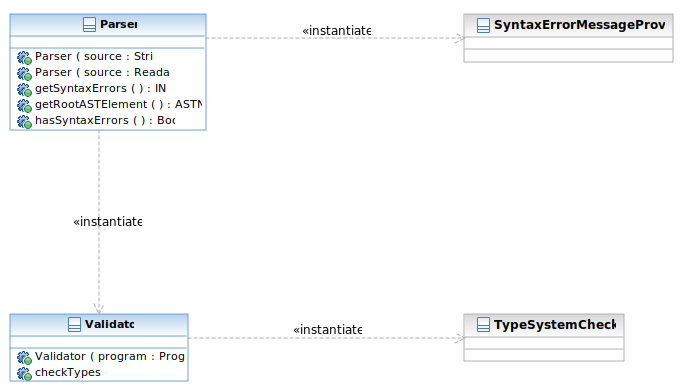
\includegraphics[width=\textwidth]{diagrams/parser_component.pdf}
